\subsection{Firm Characteristics Data}

In this paper, we deviate from the traditional approach of constructing all variables from raw data obtained from databases like Compustat or Thomson Reuters. Instead, we utilize firm characteristic data from Open Source Asset Pricing\footnote{The dataset consists of 319 characteristics that are based on previous asset pricing studies. Out of these, 161 characteristics exhibit significant t-statistics when compared to the original papers, while 44 show mixed evidence and the remaining 114 are found to be insignificant. From the 161 variables that show significant t-statistics, we select our firm characteristic variables based on variable importance discussed in the existing literature while also considering data completeness, in order to minimize the number of missing values in the dataset. The database is maintained and updated annually by the authors, and open-source code is provided for the purpose of enhancing the reproducibility.}, a dataset created and maintained by \citet*{chen2021open}. There are several reasons for this decision. First, machine learning papers typically involve analyzing a large number of feature variables, which can be time-consuming to construct. For instance, \citet*{kozak2020shrinking} used 50 anomaly characteristics and 80 financial ratios from WRDS, while \citet*{freyberger2020dissecting} used 62 characteristics. Second, constructing these feature variables based on the original paper's descriptions requires a meticulous approach, and even small subjective variations can lead to different datasets. Third, using a self-constructed dataset can make reproducing the paper more challenging and reduce comparability with other machine learning papers.

We do not corperate all the variables from the dataset in our analysis, instead only part of variables are selected for the study.The selection of firm characteristic variables for our empirical research is guided by the existing literature on the variables' relevance in predicting stock return, as well as by the completeness of each variable in avoiding the inclusion of too many missing values, which is related with our approach of handling missing values, thereby ensuring a maximally sized dataset. \citet*{gu2020empirical}, \citet*{leippold2022machine}, and \citet*{drobetz2021empirical} replace all missing values with the cross-sectional median of each firm characteristic variables in that month. Although, This approach allow us to include as many firm characteristic variables as we want, it needs strong assumptions on the structure of the data and creates artificial time-series fuctuation in the firm characteristics variables. Given the non-random nature of missing data in firm characteristics, as noted by \citet*{bryzgalova2022missing}, we choose not to use artificial imputation methods, instead opting to drop all missing values to obtain a balanced dataset. In such a way to aviod additional source of errors and keep the dependency structure in the dataset. Our final selection includes 49 firm characteristic variables categorized into 7 categories, namely "Value", "Investment", "Trading", "Profitability", "Momentum", "Intangible", and "Risk", which are similar to those used by \citet*{chen2019deep} as presented in Table \ref{table: Firm Characteristics by Category}. Notably, the Open Source Asset Pricing database does not provide the variables "short-term reversal", "size", and "return", which we abtain from the Center for Research in Security Prices (CRSP) and merge using the unique stock identifier PERMNO and date.

\begin{table}[H]
  \footnotesize
  \centering
  \caption{Firm Characteristics by Category}
  \label{table: Firm Characteristics by Category}
  \begin{tabularx}{\linewidth}{ ll >{\setlength\hsize{11\hsize}} X ll>{\setlength\hsize{11\hsize}} X}
  \cline{1-6}
  ~ & \textbf{Value} & ~ & ~ & \textbf{Moment} \\\cline{2-3} \cline{5-6}
  1 & AssetGrowth & Asset growth & 27 & LRreversal & Long‐run reversal \\
  2 & Size & Size & 28 & STreversal & Short term reversal \\
  3 & SP & Sales‐to‐price & 29 & Mom12m & Momentum (12 month) \\
  4 & NOA & Net Operating Assets & 30 & Mom6m & Momentum (6 month) \\
  5 & AM & Total assets to market & 31 & MRreversal & Medium‐run reversal \\
  6 & ChEQ & Growth in book equity & 32 & IntMom & Intermediate Momentum \\
  7 & DelEqu & Change in equity to assets & 33 & ResidualMomentum & Momentum based on FF3 residuals \\
  8 & ChNWC & Change in Net Working Capital & ~ & ~ & ~ \\
  9 & BMdec & Book to market using December ME & ~ & ~ & ~ \\
  ~ & ~ & ~ & ~ & \textbf{Risk} & ~ \\\cline{5-6}
  ~ & \textbf{Investment} & ~ & 34 & CF & Cash flow to market \\\cline{2-3}
  10 & ShareRepurchase & Share repurchases & 35 & IdioRisk & Idiosyncratic risk \\
  11 & ShareIss1Y & Share issuance (1 year) & 36 & Leverage & Market leverage \\
  12 & InvestPPEInv & change in ppe and inv/assets & 37 & BookLeverage & Book leverage (annual) \\
  13 & dNoa & change in net operating assets & 38 & IdioVol3F & Idiosyncratic risk (3 factor) \\
  14 & DelLTI & Change in long‐term investment & 39 & DelFINL & Change in financial liabilities \\
  15 & DelCOA & Change in current operating assets & 40 & cfp & Operating Cash flows to price \\
  16 & GrLTNOA & Growth in long term operating assets & 41 & DelCOL & Change in current operating liabilities \\
  ~ & ~ & ~ & ~ & ~ & ~ \\
  ~ & \textbf{Trading Frictions} & ~ & ~ & \textbf{Profitbility} & ~ \\\cline{2-3} \cline{5-6}
  17 & Price & Price & 42 & CashProd & Cash Productivity \\
  18 & Beta & CAPM beta & 43 & roaq & Return on assets (qtrly) \\
  19 & High52 & 52 week high & 44 & GP & gross profits / total assets \\
  20 & BidAskSpread & Bid‐ask spread & 45 & RoE & net income / book equity \\
  21 & VolSD & Volume Variance & ~ & ~ & ~ \\
  22 & DolVol & Past trading volume & ~ & \textbf{Intangible} & ~ \\\cline{5-6}
  23 & Illiquidity & Amihud's illiquidity & 46 & Accruals & Accruals \\
  24 & BetaFP & Frazzini‐Pedersen Beta & 47 & OPLeverage & Operating leverage \\
  25 & VolMkt & Volume to market equity & 48 & AbnormalAccruals & Abnormal Accruals \\
  26 & MaxRet & Maximum return over month & 49 & PctAcc & Percent Operating Accruals \\
  \hline
  \end{tabularx}
\end{table}

\subsection{Macroeconomic Data}
\label{sec: macro data}
We choose CFNAI (Chicago Fed National Activity Index) index to proxy the macroeconomic conditions, as it is a commonly used measure of overall macroeconomic conditions in the US. The CFNAI is reported monthly by the Federal Reserve Bank of Chicago and is often used as a leading indicator of economic growth or recession. It is a widely followed measure in both academic and policy circles. The comprehensive CFNAI index is plotted in figure \ref{fig: CFNAI index} and the subsectional macroeconomic indices including Production and income; Employment, unemployment, and hours; Personal consumption and housing; Sales, orders, and inventories which are detailed in Appendix \ref{sec:appendixa} and presented in Figure \ref{fig: Subsectional Macroeconomic index} together with NBER suggested recession indicators.

\begin{figure}[H]
  \centering
  \caption{\textbf{CFNAI index}}
  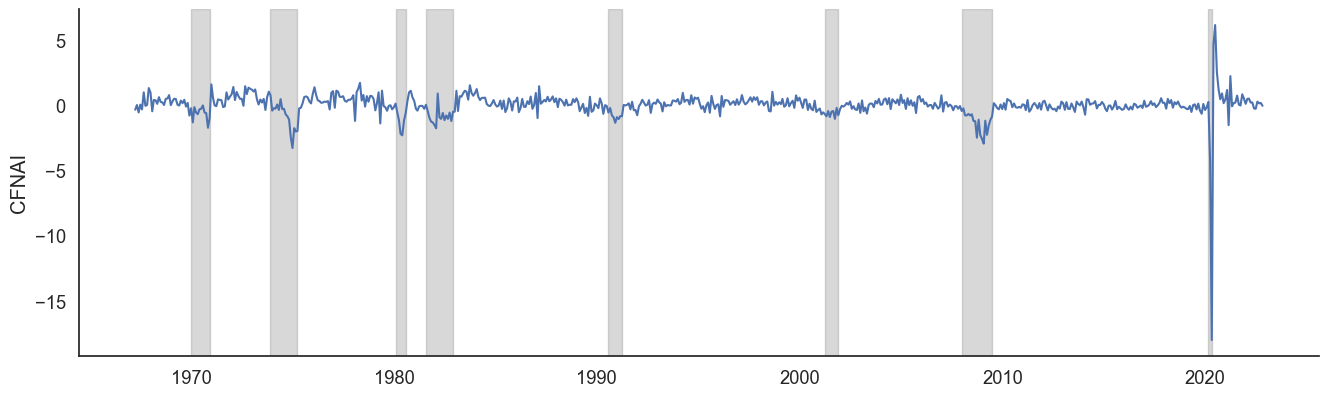
\includegraphics[width=.8\textwidth]{images/cfnai.png}
  \label{fig: CFNAI index}
  \caption*{\footnotesize{This graphic plots the historical CFNAI index from 1965 to 2022 together with NBER suggested recession periods, in 2020 the CFNAI index fell sharply due to the economic impact of the COVID-19 pandemic.}}
\end{figure} 

\subsection{Market Sentiment}
For additional analysis, we also use market sentiment data to capture the overall macroeconomic conditions. \citet*{baker2007investor} find that market sentiment, or the overall attitude of investors towards the market, can have a significant impact on stock returns. To measure market sentiment, they construct a sentiment index based on five indicators covering a wide range of measures of investor sentiment. The historical trend chart of investors sentiment is plotted in figure \ref{fig: sentiment index}, and the 5 components for constructing the investors sentiment index are also plotted in figure \ref{fig: 5 components for sentiment} in Appendix \ref{sec:appendixa2}.

\begin{figure}[H]
  \centering
  \caption{\textbf{Investors Sentiment}}
  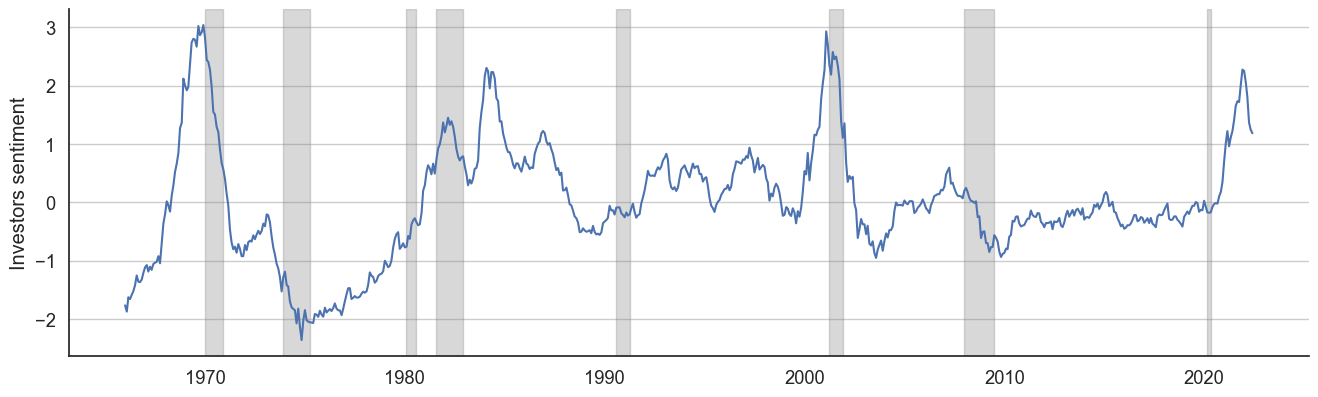
\includegraphics[width=.8\textwidth]{images/sentiment.png}
  \label{fig: sentiment index}
  \caption*{\footnotesize{Data are generally as used and described in the paper \citet*{baker2007investor} and \citet*{baker2006investor}.}}
\end{figure} 

\subsection{Fama-French 5 Factor Data}

In this study, the Fama-French 5 factor dataset and risk-free rate are incorporated from the Fama-French data library and merged with the primary dataset. A summary of the variables can be found in Table \ref{table: Fama-French 5 factor}, while an in-depth discussion on their construction and economic rationale can be found in \citet*{fama2015five} work. The collected data spans from July 1963 to the present, with a monthly frequency.

\begin{table}[H]
  \centering
  \footnotesize
  \caption{\textbf{Fama-French 5 Factor}}
  \label{table: Fama-French 5 factor}
  \begin{tabular}{l>{\RaggedRight}p{0.8\linewidth}}
  \hline
      \textbf{Acronym} & \textbf{Defination} \\ \hline
      SMB & SMB (Small Minus Big) is the average return on the nine small stock portfolios minus the average return on the nine big stock portfolios. \\ 
      HML & HML (High Minus Low) is the average return on the two value portfolios minus the average return on the two growth portfolios. \\ 
      RMW & RMW (Robust Minus Weak) is the average return on the two robust operating profitability portfolios minus the average return on the two weak operating profitability portfolios.  \\ 
      CMA & CMA (Conservative Minus Aggressive) is the average return on the two conservative investment portfolios minus the average return on the two aggressive investment portfolios. \\ 
      Mkt-RF & Rm-Rf, the excess return on the market, value-weight return of all CRSP firms incorporated in the US and listed on the NYSE, AMEX, or NASDAQ that have a CRSP share code of 10 or 11 at the beginning of month t, good shares and price data at the beginning of t, and good return data for t minus the one-month Treasury bill rate (from Ibbotson Associates). \\ 
      RF & One-month Treasury bill rate (from Ibbotson Associates). \\ \hline
  \end{tabular}
  \begin{tablenotes}
    \small
    \item The Fama/French 5 factors (2x3) are constructed using the 6 value-weight portfolios formed on size and book-to-market, the 6 value-weight portfolios formed on size and operating profitability, and the 6 value-weight portfolios formed on size and investment.
  \end{tablenotes}
\end{table}

\subsection{Abnormal Return}

The purpose of this study is to compare the performance of neural network models in predicting different measures of stock return. Specifically, we focus on stock excess return, which is defined as the actual stock return minus the one-month Treasury bill rate, and we construct stock abnormal return using the methodology of \citet*{kaniel2022machine}. To be precise, we define the abnormal return for each stock as the difference between the actual excess return and the expected return based on factor models, i.e., the alpha of the factor models.

Over the years, the field of finance has witnessed significant changes in the prevalence of factor models used for pricing assets. Starting from the classic Capital Asset Pricing Model (CAPM) introduced by \citet*{sharpe1964capital}, the evolution of asset pricing models led to the Intertemporal Capital Asset Pricing Model (ICAPM) by \citet*{merton1973intertemporal}. The Fama-French Three-Factor Model (FF3) proposed by \citet*{fama1992cross} gained popularity for being able to better explain the cross-section of stock returns than the CAPM. However, it has since been replaced by the more recent Fama-French Five-Factor Model (FF5) introduced by the same authors \citet*{fama2015five}. Moreover, researchers have proposed unofficial extensions to the FF5 model, such as the Fama-French Five-Factor Model with Momentum (FF5F+M) and the Fama-French Six-Factor Model (FF6), which includes a volatility factor, as suggested in a paper by \citet*{harvey2016and}. To ensure the study covers the historical trend without drifting too much from the main academic consensus, we aim to compare the abnormal returns obtained using CAPM, FF3, and FF5 models, given the long time horizon of our analysis spanning over five decades.

Specifically, we first require that each stock has at least 37 observations and estimate betas for each of the factors over the past 36 months, using equation \ref{eqn:abnormal return 1} as presented below:

\begin{equation}
  \label{eqn:abnormal return 1}
  R_{i,t-36:t} = \alpha_{i,t-36:t} + F_{t-36:t} \hat{\beta}_{i,t} + \epsilon_{i, t-36:t}
\end{equation}

\noindent in which $R_{i,t}$ is the return of stock $i$ in month $t$ in excess of a one-month risk-free rate, $F_t$ is a vector of factors, take Fama-French 5 factors model as an example, $F_t$ would be $[SMB_t + HML_t + RMW_t + CMA_t + (R_m - R_f)_t]$, and $\hat{\beta}_{i,t}$ is a vector of estimated coefficients accordingly. Then, we use the estimated $\hat{\beta}_{i,t}$ from the past 36 months to predict the stock return for 37th month $R^E_{i,t+1} = F_{t+1}\hat{\beta}_{i,t}$. Finally, the abnormal return for the stock is obtained as the difference between the actual excess return and the Fama-French 5 factors' expected return, using equation \ref{eqn:abnormal return 2}.

\begin{equation}
  \label{eqn:abnormal return 2}
  R^{abn}_{i,t+1} = R_{i,t+1} - R^E_{i,t+1}
\end{equation}

Figure \ref{fig: abnormal_excess_return} presents a graphical representation of the key features of stock excess and abnormal returns. The left panel showcases the cumulative monthly average excess and abnormal returns, together with the shaded NBER suggested recession periods. The cumulative excess return displays a clear upward slope, indicating a considerable increase of over four times high from the first to the last month. And several drawdowns happend during or next to the NBER suggested recession periods. In contrast, the cumulative abnormal returns from the CAPM model oscillate within the range of [0,1], whereas those from the 3- and 5-factor models fluctuate within the range of [-1,0]. Nevertheless, some drawdowns in the cumulative monthly average abnormal returns coincide with the NBER suggested recession periods. Among stock abnormal returns derived from different factor models, the abnormal return generated by the 5-factor model deviates the least from zero line, suggesting that it is the best factor model for predicting stock returns among other factor models.

The right panel of Figure \ref{fig: abnormal_excess_return} displays the monthly standard deviation of stock excess and abnormal returns. Most of the time, the monthly standard deviation of excess and abnormal stock returns overlap with each other. However, there is a peak in abnormal returns from the 5-factor model around 2004 that cannot be explained. We also provide a summary of the statistics for various measurements of stock returns in Appendix Table \ref{table: Summary statistic of return}, as well as a heatmap in Figure \ref{fig: abnormal_excess_corr} illustrating their correlations.

\begin{figure}[H]
  \centering
  \caption{\textbf{Cumulative Excess and Abnormal Return}}
  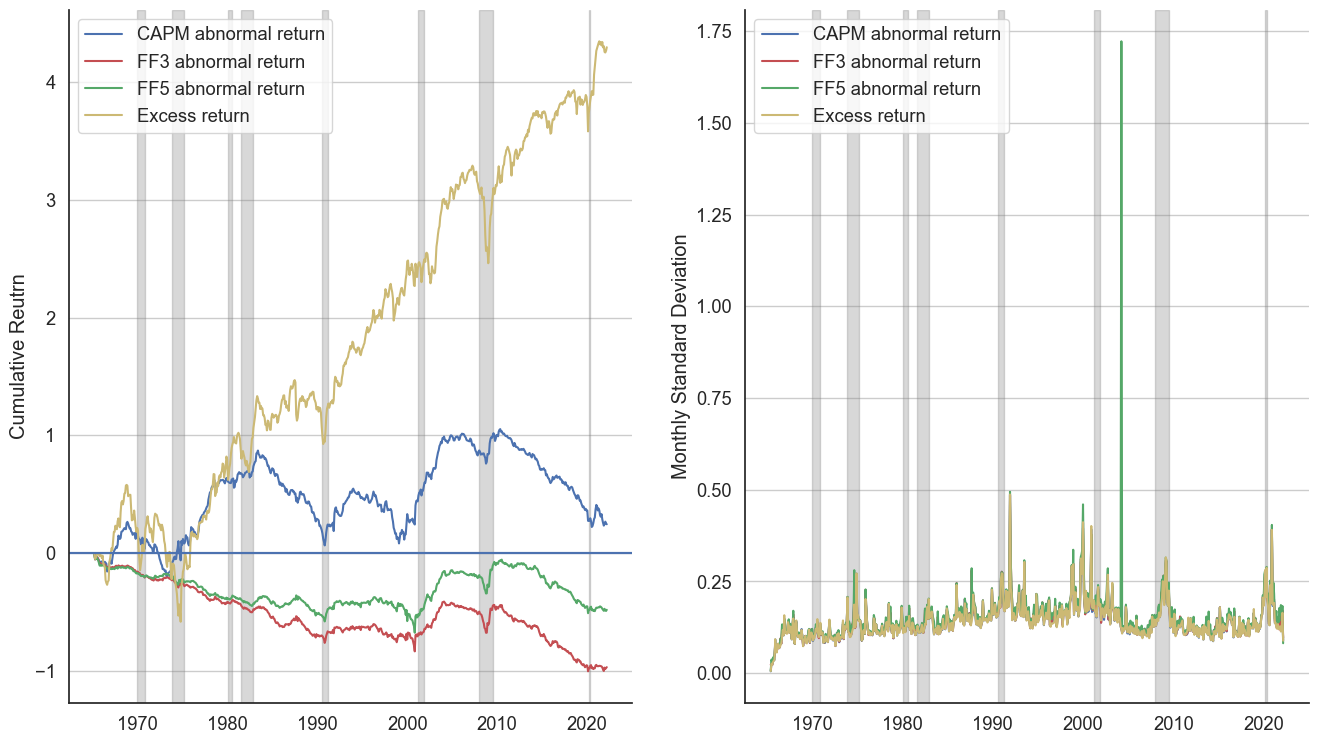
\includegraphics[width=.8\textwidth]{images/abnormal_excess_return.png}
  \label{fig: abnormal_excess_return}
  \caption*{\footnotesize{The left panel of this figure shows the monthly average excess and abnormal return accumulated for the whole time period in our dataset. The left panel presents the standard deviation of stock excess and abnormal returns in each month.}}
\end{figure} 

\subsection{Related to Neural Network}

To ensure that the neural network model is trained on a balanced dataset, it is important to handle missing values carefully. Previous studies such as \citet*{gu2020empirical} and \citet*{gu2019autoencoder} have used the cross-sectional median for each feature variable during the respective month to replace the missing values. However, this approach introduces artificial data and may compromise the dependency structure, resulting in additional errors. To address this issue, we adopt the approach of \citet*{kelly2019characteristics} and \citet*{chen2019deep}, which involves dropping all the missing observations from the dataset. This also explains why we do not include all 161 variables from the database. The resulting dataset for firm characteristics contains more than 10,000 companies with over 1,100,000 observations. The sample period covers stocks from December 1971 to December 2021, spanning a total of 50 years.

One commonly used methodology for sample splitting in studies, as demonstrated in works such as \citet*{kozak2020shrinking}, \citet*{gu2020empirical}, and \citet*{chen2019deep}, is to split the data chronologically. This approach, for example, usually allocating the initial 20 years for the training dataset, the subsequent 10 years for validation, and the final 20 years for testing. However, in this study, we adopt a different approach based on the methodology proposed by \citet*{kaniel2022machine}. We divide the full sample into three subsamples of equal length randomly. The first sample is utilized as the training dataset to estimate the neural network model. The second sample serves as the validation dataset to tune the hyperparameters, such as the depth of the model, number of nodes in each layer, choice of learning rate, and regularization penalties. The final sample is reserved as the test dataset to evaluate the performance of out-of-sample predictions. The random sampling of the dates is predicted  on the assumption that the mapping function between stock returns and the conditioning information variables is independent over time, akin to strict cross-section asset pricing analyses.

The methodology used for sample splitting in our study is crucial for three reasons. Firstly, it enables us to conduct an analysis of the impact of macroeconomic conditions on stock returns. Certain macroeconomic conditions, such as low CFNAI index values during recession periods, are only present in a small subset of the data and may be overlooked in conventional chronological data splitting. Secondly, the performance of the neural network model can be severely impacted if there is any unobserved time trend. By using the random sample splitting methodology, all periods of the data are evenly distributed in the training, validation, and test datasets, allowing the model to learn from data across all time periods even if some important variables are not included in the dataset. This methodology ensures that our model can provide reliable predictions. Lastly, the use of the random sample splitting method allows us to use data from all time periods for the out-of-sample analysis, diminishing the effect of specific subperiods. If we follow the conventional chronological sample splitting methodology, the evaluation would only focus on the shorter last part of the data, potentially ignoring important information from earlier periods.

As discussed in Section \ref{sec:neural network}, we select the mean squared error as our objective function to optimize the weights and the rectified linear unit (ReLU) as the activation function to capture the non-linear transformations from the input to hidden layers. We utilize the 'He initializer' to avoid the problem of "dying ReLU". The maximum number of epochs during each training process was set to 100, and early stopping was implemented based on the R-Squared value in the validation dataset.

To enhance the stability of the training process, we use batch normalization, and to improve the robustness of our predictions, we employe ensembled learning by combining the predictions of 10 models. The detailed model specifications are presented in Table \ref{table: model summary}, and the optimal network architecture comprises one hidden layer with 32 hidden nodes. The other hyperparameters are tuned using the validation dataset and are listed in the left panel of the table.

\begin{table}[H]
  \centering
  \caption{\textbf{Model Summary}}
  \begin{tabular}{lllll}
  \hline
      \multicolumn{3}{c}{Tunning Parameters} & \multicolumn{2}{c}{Other Parameters}\\ \cline{4-5}
      Parameters & Candidates & Final Model & Objective Function & MSE \\ \cline{1-3}
      Hidden Layers  & 1, 2, 3 & 1 & Activation Function  & ReLU \\ 
      Hidden Nodes  & 32 , 16, 4 & 32 & Kernel Initializer & He Initializer \\ 
      Learning Rate & 0.01, 0.001 & 0.01 & Ensembled Models & 10 \\ 
      Decay Rate & 0.01, 0.001 & 0.001 & Maximum Epochs & 100 \\ 
      Momentum & 0.95, 0.99 & 0.99 & Early Stop Monitor  & Validation R2 \\ 
      L1 Weight Penalty & 0.001, 0.005 & 0.005 & Early Stop Patience & 10 \\ 
      Batch Size  & 3200, 32000 & 3200 & Batch Normalization & Applied \\ \hline
  \end{tabular}
  \label{table: model summary}
\end{table}

